\chapter{Permukaan, Adsorpsi, dan Katalisis Heterogen}\label{ch:b3:surfaces-catalysis}

Di bawah sebuah mobil, di dalam kaleng baja, terdapat sarang lebah keramik
yang ribuan salurannya dilapisi oksida berpori yang memuat beberapa gram
platina, paladium, dan rodium. Dalam sepersekian detik, gas buang yang
mengalir melaluinya kehilangan sebagian besar karbon monoksida, hidrokarbon
yang tidak terbakar, dan nitrogen oksidanya. Tidak ada yang terjadi di dalam
gas: setiap reaksi itu berlangsung di permukaan partikel logam yang
berukuran beberapa nanometer. Sebagian besar industri kimia bekerja dengan
cara yang sama, dari amonia untuk pupuk sampai perengkahan minyak bumi. Bab ini
menjelaskan bagaimana molekul melekat pada permukaan, seberapa luas permukaan
yang ditutupinya, bagaimana reaksi permukaan berlangsung, dan bagaimana
katalis padat dibuat, diukur, dan diamati.

\begin{recall}
Jilid Tahun 1 mendefinisikan katalis serta perbedaan antara katalisis homogen
dan katalisis heterogen, dan menjelaskan susunan kubus berpusat muka pada
logam. Jilid Tahun 2 mendefinisikan konversi, selektivitas, dan frekuensi
pergantian sebuah katalis, serta asas Le Chatelier.
\Cref{ch:b3:x-ray-diffraction} memperkenalkan \omterm{def:b3:x-ray-diffraction:miller}{indeks Miller},
\cref{ch:b3:rate-theories} \omterm{thm:b3:rate-theories:eyring}{persamaan Eyring}, dan
\cref{ch:b3:partition-functions} statistika distribusi.
\end{recall}

\begin{omfigure}
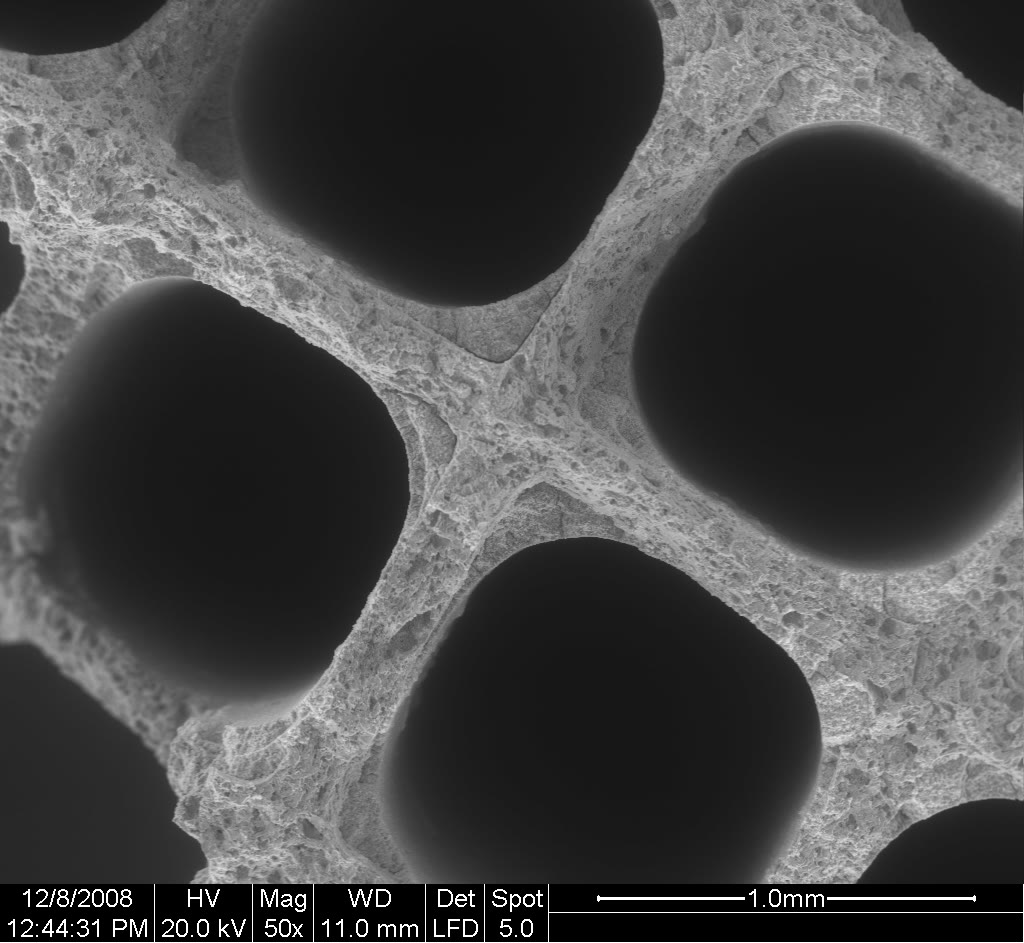
\includegraphics[width=0.48\linewidth]{images/book4/converter-sem.jpg}

{\small Sarang lebah keramik sebuah konverter katalitik yang dilihat dengan
mikroskop elektron pemindai (batang skala \qty{1.0}{mm}): saluran-saluran
persegi yang dipisahkan oleh dinding tipis berpori, yang membawa lapisan
oksida beserta partikel-partikel logamnya.}
\end{omfigure}

\section{Adsorpsi}

\begin{definition}[Adsorpsi]\label{def:b3:surfaces-catalysis:adsorption}
Yang disebut \emph{adsorpsi}\index{adsorpsi} adalah penumpukan molekul gas atau
zat terlarut pada permukaan padatan atau cairan. Molekul yang teradsorpsi
disebut \emph{adsorbat}\index{adsorbat}, padatannya \emph{adsorben}\index{adsorben};
proses kebalikannya adalah \emph{desorpsi}\index{desorpsi}.
\end{definition}

\begin{definition}[Fisisorpsi, kemisorpsi]\label{def:b3:surfaces-catalysis:physi-chemi}
Yang disebut \emph{fisisorpsi}\index{fisisorpsi} adalah \omterm{def:b3:surfaces-catalysis:adsorption}{adsorpsi} oleh gaya van der
Waals, dengan entalpi \omterm{def:b3:surfaces-catalysis:adsorption}{adsorpsi} paling besar beberapa puluh kilojoule per mol,
yang sebanding dengan entalpi kondensasi, dan tanpa perubahan pada molekulnya.
Pada \emph{kemisorpsi}\index{kemisorpsi} terbentuk ikatan kimia dengan permukaan,
dengan entalpi sekitar 40 sampai beberapa ratus kilojoule per mol; kemisorpsi
dapat memecah molekul (kemisorpsi disosiatif) dan berhenti pada satu lapisan.
\end{definition}

\begin{omfigure}
\begin{tikzpicture}[font=\small, >=Stealth, x=1cm, y=1cm]
  \draw[->] (0,-2.6) -- (0,1.8) node[anchor=south] {energi};
  \draw[->] (0,0) -- (8.0,0) node[anchor=south east] {jarak dari permukaan};
  \draw[omDef, thick] plot[smooth, tension=0.7] coordinates {(1.6,1.6) (2.2,-0.25) (2.8,-0.62) (3.6,-0.35) (5.0,-0.08) (7.5,0)};
  \draw[omThm, thick] plot[smooth, tension=0.6] coordinates {(0.45,1.6) (0.8,-1.2) (1.2,-2.2) (1.7,-1.6) (2.35,-0.15) (2.9,0.9) (3.5,1.5)};
  \node[omDef, anchor=north west, font=\scriptsize] at (3.4,-0.4) {\ce{H2} terfisisorpsi (prekursor)};
  \node[omThm, anchor=west, font=\scriptsize] at (1.75,-1.9) {2 H terkemisorpsi};
  \node[omThm, anchor=west, font=\scriptsize, align=left] at (3.55,1.45) {menuju $\mathrm{H} + \mathrm{H}$\\ jauh dari permukaan};
  \fill (2.3,-0.2) circle (1.5pt);
  \node[font=\scriptsize] (cr) at (2.5,1.85) {persilangan};
  \draw[black!60] (cr.south) -- (2.3,-0.12);
\end{tikzpicture}

{\small Energi potensial molekul hidrogen yang mendekati permukaan logam
(skematis). Molekul itu mula-mula jatuh ke dalam sumur \omterm{def:b3:surfaces-catalysis:physi-chemi}{fisisorpsi} yang dangkal;
di tempat kurva ini memotong kurva dua atom H yang masing-masing terikat,
molekul itu dapat terdisosiasi ke dalam sumur \omterm{def:b3:surfaces-catalysis:physi-chemi}{kemisorpsi} yang dalam. Jika
persilangan itu terletak di atas nol, \omterm{def:b3:surfaces-catalysis:physi-chemi}{kemisorpsi} disosiatif itu teraktivasi.}
\end{omfigure}

Permukaan partikel logam sebagian besar memperlihatkan muka-muka kisi fcc yang
paling rapat, (111) dan (100). Pada muka itu, \omterm{def:b3:surfaces-catalysis:adsorption}{adsorbat} dapat duduk di atas satu
atom (puncak), di antara dua atom (jembatan), atau di dalam rongga di antara
tiga atau empat atom, dan energi ikatnya berbeda dari satu situs ke situs lain.

\begin{omfigure}
\begin{tikzpicture}[font=\scriptsize]
  % fcc(111): lapisan heksagonal, jarak 0.6 cm
  \foreach \i in {0,...,5}{\foreach \j in {0,...,4}{
    \shade[ball color=black!25] ({0.6*\i+0.3*\j},{0.52*\j}) circle (0.29);}}
  \fill[omThm] (1.2+0.3*1,0.52) circle (0.07);
  \fill[omDef] ({0.6*2+0.3*2+0.3},{0.52*2}) circle (0.07);
  \fill[black] ({0.6*3+0.3*2+0.3},{0.52*2+0.17}) circle (0.07);
  \fill[black!60!green] ({0.6*1+0.3*3+0.3},{0.52*3-0.17}) circle (0.07);
  \node[anchor=north] at (2.1,-0.45) {fcc(111)};
  % fcc(100): lapisan persegi
  \begin{scope}[xshift=5.6cm]
  \foreach \i in {0,...,4}{\foreach \j in {0,...,4}{
    \shade[ball color=black!25] ({0.6*\i},{0.6*\j}) circle (0.29);}}
  \fill[omThm] (1.2,1.2) circle (0.07);
  \fill[omDef] (1.5,1.8) circle (0.07);
  \fill[black] (2.1,0.9) circle (0.07);
  \node[anchor=north] at (1.2,-0.45) {fcc(100)};
  \end{scope}
  \node[anchor=west, align=left] at (9.0,1.6) {\textcolor{omThm}{$\bullet$} puncak\\ \textcolor{omDef}{$\bullet$} jembatan\\
    $\bullet$ rongga (lipat 3 atau 4)\\ \textcolor{black!60!green}{$\bullet$} rongga lipat 3 kedua (111)};
\end{tikzpicture}

{\small Tampak atas dua muka paling rapat sebuah logam kubus berpusat muka,
beserta situs-situs \omterm{def:b3:surfaces-catalysis:adsorption}{adsorpsinya}: di puncak satu atom, menjembatani dua atom,
dan di dalam rongga di antara tiga atom pada (111) (dua jenis, di atas sebuah
atom lapisan kedua atau tidak) atau empat atom pada (100).}
\end{omfigure}

\begin{definition}[Fraksi tutupan, lapisan tunggal]\label{def:b3:surfaces-catalysis:coverage}
Yang disebut \emph{fraksi tutupan}\index{fraksi tutupan} $\theta$ sebuah permukaan
adalah fraksi situs \omterm{def:b3:surfaces-catalysis:adsorption}{adsorpsinya} yang terisi. Yang disebut
\emph{lapisan tunggal}\index{lapisan tunggal} adalah satu lapisan \omterm{def:b3:surfaces-catalysis:adsorption}{adsorbat} yang lengkap, $\theta = 1$.
\end{definition}

\section{Isoterm}

\begin{theorem}[Isoterm Langmuir]\label{thm:b3:surfaces-catalysis:langmuir}
Jika sebuah permukaan memiliki situs-situs yang identik dan saling bebas, yang
masing-masing menampung satu molekul, tutupan pada kesetimbangan dengan gas
bertekanan $p$ adalah
\[
  \theta = \frac{Kp}{1 + Kp},
\]
dengan $K$, tetapan kesetimbangan \omterm{def:b3:surfaces-catalysis:adsorption}{adsorpsi}, yang hanya bergantung pada suhu.
Inilah \emph{isoterm Langmuir}\index{isoterm Langmuir}.
\end{theorem}

\begin{proof}
Bukti kinetik. Molekul teradsorpsi pada situs-situs bebas dengan laju $k_ap(1 - \theta)N$ ($N$
situs) dan terdesorpsi dengan laju $k_d\theta N$. Pada kesetimbangan keduanya sama: $\theta/(1 - \theta)
= (k_a/k_d)p$, yang setelah disusun ulang memberikan hasil itu dengan $K = k_a/k_d$.

Bukti statistik. $M$ molekul pada $N$ situs dapat disusun dengan $N!/(M!(N - M)!)$ cara,
dan setiap molekul yang teradsorpsi memiliki fungsi partisi internal $q_{\mathrm s}$
(vibrasinya terhadap permukaan dan energi ikatnya). Dengan rumus Stirling,
potensial kimia molekul yang teradsorpsi adalah $\mu_{\mathrm s} = -kT\ln\bigl(q_{\mathrm s}\frac{1 - \theta}{\theta}\bigr)$;
potensial kimia gas ideal adalah $\mu_{\mathrm g} = \mu_{\mathrm g}^\circ + kT\ln(p/p^\circ)$. Kesetimbangan, $\mu_{\mathrm s} = \mu_{\mathrm g}$, memberikan
$\theta/(1 - \theta) = q_{\mathrm s}\eu^{\mu_{\mathrm g}^\circ/kT}p/p^\circ$: hukum yang sama, dengan $K$ dinyatakan dalam
fungsi-fungsi partisi.
\end{proof}

Pada tekanan rendah $\theta \approx Kp$ (rezim Henry); pada tekanan tinggi $\theta \to 1$.
Tutupannya setengah pada $p = 1/K$.

\begin{proposition}[Adsorpsi disosiatif]\label{prop:b3:surfaces-catalysis:dissociative}
Untuk gas diatomik yang terdisosiasi pada dua situs, $\mathrm{H_2} + 2\,{*} \to 2\,\mathrm{H}{*}$ (${*}$: sebuah situs bebas),
\[
  \theta = \frac{(Kp)^{1/2}}{1 + (Kp)^{1/2}},
\]
sehingga $\theta \propto \sqrt p$ pada tekanan rendah.
\end{proposition}

\begin{proof}
\omterm{def:b3:surfaces-catalysis:adsorption}{Adsorpsi} memerlukan dua situs bebas, dengan laju $k_ap(1 - \theta)^2$; \omterm{def:b3:surfaces-catalysis:adsorption}{desorpsi} memerlukan dua
atom teradsorpsi yang bergabung kembali, dengan laju $k_d\theta^2$. Kesamaan keduanya memberikan $\theta/(1 - \theta) =
(Kp)^{1/2}$.
\end{proof}

\begin{proposition}[Adsorpsi kompetitif]\label{prop:b3:surfaces-catalysis:competitive}
Dua gas A dan B yang bersaing memperebutkan situs yang sama menutupinya dengan
\[
  \theta_{\mathrm A} = \frac{K_{\mathrm A}p_{\mathrm A}}{1 + K_{\mathrm A}p_{\mathrm A} + K_{\mathrm B}p_{\mathrm B}}, \qquad
  \theta_{\mathrm B} = \frac{K_{\mathrm B}p_{\mathrm B}}{1 + K_{\mathrm A}p_{\mathrm A} + K_{\mathrm B}p_{\mathrm B}} .
\]
\end{proposition}

\begin{proof}
Untuk setiap gas, $k_{a,\mathrm A}p_{\mathrm A}(1 - \theta_{\mathrm A} - \theta_{\mathrm B}) = k_{d,\mathrm A}\theta_{\mathrm A}$, dan demikian pula untuk B. Jadi
$\theta_{\mathrm A} = K_{\mathrm A}p_{\mathrm A}\theta_\ast$ dan $\theta_{\mathrm B} = K_{\mathrm B}p_{\mathrm B}\theta_\ast$ dengan $\theta_\ast = 1 - \theta_{\mathrm A} - \theta_{\mathrm B}$ sebagai fraksi bebas; dengan menjumlahkan,
$1 - \theta_\ast = \theta_\ast(K_{\mathrm A}p_{\mathrm A} + K_{\mathrm B}p_{\mathrm B})$.
\end{proof}

\begin{definition}[Entalpi adsorpsi isosterik]\label{def:b3:surfaces-catalysis:isosteric}
Yang disebut \emph{entalpi adsorpsi isosterik}\index{entalpi adsorpsi isosterik}
$\Delta_{\mathrm{ads}}H$ adalah entalpi molar \omterm{def:b3:surfaces-catalysis:adsorption}{adsorpsi} pada tutupan yang tetap,
yang diperoleh dari tekanan-tekanan yang memberikan tutupan yang sama pada
suhu-suhu yang berbeda.
\end{definition}

\begin{proposition}[Entalpi isosterik]\label{prop:b3:surfaces-catalysis:isosteric}
Pada tutupan tetap,
\[
  \Bigl(\frac{\partial\ln p}{\partial T}\Bigr)_\theta = -\frac{\Delta_{\mathrm{ads}}H}{RT^2} .
\]
\end{proposition}

\begin{proof}
Pada $\theta$ tetap, $Kp$ tetap (untuk permukaan Langmuir; pada umumnya argumen yang sama
berlaku dengan tetapan kesetimbangan pada tutupan itu), sehingga $\ln p =
\text{tetapan} - \ln K$. Menurut persamaan van 't Hoff, $\dd\ln K/\dd T = \Delta_{\mathrm{ads}}H/RT^2$ (dengan $K$
yang diacukan pada sebuah tekanan standar).
\end{proof}

Karena \omterm{def:b3:surfaces-catalysis:adsorption}{adsorpsi} bersifat eksotermik, suhu yang lebih tinggi memerlukan tekanan
yang lebih tinggi untuk tutupan yang sama: isoterm-isoterm pada gambar menurun
ketika $T$ naik.

\begin{theorem}[Isoterm BET]\label{thm:b3:surfaces-catalysis:bet}
Jika molekul teradsorpsi dalam lapisan-lapisan yang berurutan, lapisan pertama
dengan tetapan ikat yang khas bagi permukaannya dan lapisan-lapisan lainnya
dengan kesetimbangan kondensasi cairannya, jumlah yang teradsorpsi pada
tekanan relatif $x = p/p^*$ ($p^*$: tekanan uap \omterm{def:b3:surfaces-catalysis:adsorption}{adsorbat} cair) adalah
\[
  \frac{v}{v_{\mathrm m}} = \frac{cx}{(1 - x)(1 - x + cx)},
\]
dengan $v_{\mathrm m}$ jumlah dalam satu \omterm{def:b3:surfaces-catalysis:coverage}{lapisan tunggal} dan $c$ sebuah tetapan
yang berkaitan dengan selisih antara entalpi \omterm{def:b3:surfaces-catalysis:adsorption}{adsorpsi} pada lapisan pertama dan
entalpi kondensasi. Inilah \emph{isoterm BET}\index{isoterm BET} (Brunauer,
Emmett, dan Teller).
\end{theorem}

\begin{proof}
Misalkan $s_i$ fraksi permukaan yang tertutup oleh tepat $i$ lapisan. Neraca
setiap lapisan, seperti pada bukti Langmuir, memberikan $s_1 = cxs_0$ dan $s_i =
xs_{i-1}$ untuk $i \ge 2$, sehingga $s_i = cx^is_0$. Jumlah yang teradsorpsi adalah $v/v_{\mathrm m} =
\sum_iis_i/\sum_is_i$. Dengan $\sum_{i\ge1}x^i = x/(1 - x)$ dan $\sum_{i\ge1}ix^i = x/(1 - x)^2$:
\[
  \frac{v}{v_{\mathrm m}} = \frac{cs_0\,x/(1 - x)^2}{s_0[1 + cx/(1 - x)]} = \frac{cx}{(1 - x)(1 - x + cx)} .
\]
\end{proof}

Setelah disusun ulang, $\dfrac{x}{v(1 - x)} = \dfrac{1}{v_{\mathrm m}c} + \dfrac{c - 1}{v_{\mathrm m}c}\,x$: sebuah garis lurus yang kemiringan dan
perpotongannya memberikan $v_{\mathrm m}$ dan $c$, yang biasanya berlaku untuk $0.05 < x < 0.30$.

\begin{definition}[Luas permukaan spesifik]\label{def:b3:surfaces-catalysis:surface-area}
Yang disebut \emph{luas permukaan spesifik}\index{luas permukaan spesifik} sebuah padatan adalah
luas permukaannya per satuan massa, termasuk dinding pori-porinya.
\end{definition}

\begin{method}[Luas permukaan spesifik dari isoterm nitrogen]\label{met:b3:surfaces-catalysis:bet-area}
\begin{enumerate}
  \item Hilangkan gas dari sampel dalam vakum sambil dipanaskan; dinginkan sampel
        itu dalam nitrogen cair (\qty{77}{K}).
  \item Ukurlah volume nitrogen yang teradsorpsi (dikonversi ke kondisi standar)
        pada tekanan relatif antara 0.05 dan 0.30.
  \item Alurkan $x/(v(1 - x))$ terhadap $x$; dari kemiringan dan perpotongannya,
        $v_{\mathrm m} = 1/(\text{kemiringan} + \text{perpotongan})$ dan $c = 1 + \text{kemiringan}/\text{perpotongan}$.
  \item Luas $= n_{\mathrm m}N_Aa_{\mathrm m}$, dengan $n_{\mathrm m}$ jumlah dalam \omterm{def:b3:surfaces-catalysis:coverage}{lapisan tunggal} dan $a_{\mathrm m} = \qty{0.162}{nm^2}$
        luas konvensional sebuah molekul nitrogen yang teradsorpsi.
\end{enumerate}
\end{method}

\begin{omfigure}
\begin{tikzpicture}
\begin{axis}[name=la, width=0.31\linewidth, height=5.0cm, xmin=0, xmax=100, ymin=0, ymax=1.05,
  axis lines=left, xlabel={$p$ / kPa}, ylabel={$\theta$}, tick label style={font=\small},
  label style={font=\small}, title={\small Langmuir}]
\addplot[omDef, thick] table[x=p_kPa, y=T300] {figdata/out/bachelor-3-langmuir-bet-langmuir.dat};
\addplot[omThm, thick] table[x=p_kPa, y=T350] {figdata/out/bachelor-3-langmuir-bet-langmuir.dat};
\node[font=\scriptsize, omDef, anchor=south east] at (axis cs:98,0.92) {\qty{300}{K}};
\node[font=\scriptsize, omThm, anchor=north east] at (axis cs:98,0.45) {\qty{350}{K}};
\end{axis}
\begin{axis}[name=be, at={(la.east)}, anchor=west, xshift=1.9cm, width=0.31\linewidth, height=5.0cm,
  xmin=0, xmax=0.9, ymin=0, ymax=200, axis lines=left, xlabel={$p/p^*$},
  ylabel={$v$ / \unit{cm^3.g^{-1}}}, tick label style={font=\small}, label style={font=\small},
  title={\small BET}]
\addplot[black, thick] table[x=x, y=v] {figdata/out/bachelor-3-langmuir-bet-bet.dat};
\addplot[only marks, mark=*, mark size=1.4pt, omDef] table[x=x, y=v] {figdata/out/bachelor-3-langmuir-bet-data.dat};
\draw[black!40, dashed] (axis cs:0,45) -- (axis cs:0.9,45);
\node[font=\scriptsize, anchor=south east] at (axis cs:0.88,45) {$v_{\mathrm m}$};
\end{axis}
\begin{axis}[at={(be.east)}, anchor=west, xshift=2.1cm, width=0.31\linewidth, height=5.0cm,
  xmin=0, xmax=0.35, ymin=0, ymax=0.0085, axis lines=left, xlabel={$x = p/p^*$},
  ylabel={$x/(v(1 - x))$}, tick label style={font=\small}, label style={font=\small},
  scaled y ticks=false, yticklabel style={/pgf/number format/fixed, /pgf/number format/precision=3},
  title={\small Plot BET}]
\addplot[black, thin] table[x=x, y=y] {figdata/out/bachelor-3-langmuir-bet-line.dat};
\addplot[only marks, mark=*, mark size=1.4pt, omDef] table[x=x, y=y] {figdata/out/bachelor-3-langmuir-bet-data.dat};
\end{axis}
\end{tikzpicture}

{\small Kiri: \omterm{thm:b3:surfaces-catalysis:langmuir}{isoterm Langmuir} sebuah \omterm{def:b3:surfaces-catalysis:physi-chemi}{kemisorpsi} model ($\Delta_{\mathrm{ads}}H = \qty{-40}{kJ/mol}$) pada
dua suhu. Tengah: sebuah \omterm{thm:b3:surfaces-catalysis:bet}{isoterm BET} (model, $v_{\mathrm m} = \qty{45}{cm^3.g^{-1}}$, $c = 120$), dengan
titik-titik soal akhir pekan; lapisan-lapisannya menumpuk dan jumlahnya
menuju tak hingga di dekat $p = p^*$, tempat gasnya mengembun. Kanan: plot BET
linear dari titik-titik yang sama.}
\end{omfigure}

\section{Kinetika reaksi permukaan}

\begin{definition}[Mekanisme Langmuir--Hinshelwood dan Eley--Rideal]\label{def:b3:surfaces-catalysis:mechanisms}
Dalam \emph{mekanisme Langmuir--Hinshelwood}\index{mekanisme Langmuir--Hinshelwood}
kedua pereaksi teradsorpsi dan bereaksi di permukaan; dalam
\emph{mekanisme Eley--Rideal}\index{mekanisme Eley--Rideal} sebuah pereaksi yang
teradsorpsi bereaksi dengan molekul yang datang dari fase gas.
\end{definition}

\begin{proposition}[Laju Langmuir--Hinshelwood]\label{prop:b3:surfaces-catalysis:lh-rate}
Jika kesetimbangan-kesetimbangan \omterm{def:b3:surfaces-catalysis:adsorption}{adsorpsi} berlangsung cepat dan reaksi
permukaan antara A dan B yang teradsorpsi merupakan tahap penentu laju,
\[
  r = k\theta_{\mathrm A}\theta_{\mathrm B} = \frac{kK_{\mathrm A}p_{\mathrm A}K_{\mathrm B}p_{\mathrm B}}{(1 + K_{\mathrm A}p_{\mathrm A} + K_{\mathrm B}p_{\mathrm B})^2},
\]
yang, pada $p_{\mathrm B}$ tetap, paling besar ketika $K_{\mathrm A}p_{\mathrm A} = 1 + K_{\mathrm B}p_{\mathrm B}$ lalu menurun ketika A mendesak B keluar dari
permukaan.
\end{proposition}

\begin{proof}
Tutupan-tutupannya adalah tutupan pada \cref{prop:b3:surfaces-catalysis:competitive}. Dengan $u =
K_{\mathrm A}p_{\mathrm A}$ dan $a = 1 + K_{\mathrm B}p_{\mathrm B}$, $r \propto u/(a + u)^2$, yang turunannya $(a - u)/(a + u)^3$ lenyap pada
$u = a$.
\end{proof}

\begin{proposition}[Laju Eley--Rideal]\label{prop:b3:surfaces-catalysis:er-rate}
Jika A yang teradsorpsi bereaksi dengan B dalam fase gas,
\[
  r = k\theta_{\mathrm A}p_{\mathrm B} = \frac{kK_{\mathrm A}p_{\mathrm A}p_{\mathrm B}}{1 + K_{\mathrm A}p_{\mathrm A}},
\]
yang tumbuh bersama $p_{\mathrm A}$ sampai mencapai dataran, tanpa maksimum.
\end{proposition}

\begin{proof}
B tidak bersaing memperebutkan situs: $\theta_{\mathrm A}$ adalah tutupan Langmuir A saja, dan
lajunya sebanding dengan tutupan itu dan dengan laju tumbukan B dengan permukaan,
yang sebanding dengan $p_{\mathrm B}$.
\end{proof}

\begin{method}[LH atau ER dari ketergantungan pada tekanan]\label{met:b3:surfaces-catalysis:mechanism-from-rate}
\begin{enumerate}
  \item Ukurlah laju terhadap tekanan setiap pereaksi, sementara pereaksi yang
        lain dibuat tetap.
  \item Sebuah maksimum, lalu penurunan (orde negatif pada tekanan tinggi):
        Langmuir--Hinshelwood, pereaksi itu menginhibisi dengan menempati situs.
  \item Kenaikan sampai dataran untuk satu pereaksi dan orde satu untuk pereaksi
        yang lain pada semua tekanan: Eley--Rideal.
  \item Pastikan dengan pelabelan isotop atau spektroskopi permukaan; sebagian
        besar reaksi katalitik ternyata bertipe Langmuir--Hinshelwood.
\end{enumerate}
\end{method}

\begin{omfigure}
\begin{tikzpicture}
\begin{axis}[width=0.6\linewidth, height=5.4cm, xmin=0, xmax=10, ymin=0, ymax=0.3,
  axis lines=left, xlabel={$p_{\mathrm A}$ (tereduksi)}, ylabel={laju (tereduksi)},
  tick label style={font=\small}, label style={font=\small},
  legend style={font=\scriptsize, draw=none, at={(1.03,0.98)}, anchor=north west}, legend cell align=left]
\addplot[omDef!50, thick] table[x=pA, y=pB05] {figdata/out/bachelor-3-surface-rates.dat};
\addplot[omDef, thick] table[x=pA, y=pB1] {figdata/out/bachelor-3-surface-rates.dat};
\addplot[black, thick] table[x=pA, y=pB3] {figdata/out/bachelor-3-surface-rates.dat};
\addplot[omThm, thick, dashed] table[x=pA, y=ER] {figdata/out/bachelor-3-surface-rates.dat};
\legend{{LH, $p_{\mathrm B} = 0.5$}, {LH, $p_{\mathrm B} = 1$}, {LH, $p_{\mathrm B} = 3$}, {ER ($\times\frac14$)}}
\end{axis}
\end{tikzpicture}

{\small Laju reaksi permukaan bimolekular terhadap tekanan A
(satuan tereduksi, $K_{\mathrm A} = K_{\mathrm B} = 1$). Langmuir--Hinshelwood: setiap kurva mencapai puncak pada $K_{\mathrm A}p_{\mathrm A} =
1 + K_{\mathrm B}p_{\mathrm B}$, lalu menurun ketika A menggusur B. Eley--Rideal (putus-putus, diskalakan): sebuah dataran.}
\end{omfigure}

\begin{proposition}[Energi aktivasi semu]\label{prop:b3:surfaces-catalysis:apparent-ea}
Untuk reaksi permukaan unimolekular dengan \omterm{def:b3:surfaces-catalysis:adsorption}{adsorpsi} Langmuir, $r = k\theta = kKp/(1 + Kp)$.
Pada tutupan rendah, energi aktivasi yang terukur adalah $E_{a,\mathrm{app}} = E_a + \Delta_{\mathrm{ads}}H$; pada
tutupan tinggi nilainya $E_a$.
\end{proposition}

\begin{proof}
Pada tutupan rendah $r \approx kKp$, sehingga $\dd\ln r/\dd T = \dd\ln k/\dd T + \dd\ln K/\dd T = (E_a + \Delta_{\mathrm{ads}}H)/RT^2$.
Pada tutupan tinggi $\theta \approx 1$ dan $r \approx k$.
\end{proof}

Karena $\Delta_{\mathrm{ads}}H < 0$, reaksi pada permukaan yang tutupannya jarang tampak lebih
mudah daripada penghalang sebenarnya: menaikkan suhu mempercepat tahap
permukaan tetapi sekaligus mengosongkan permukaan.

\begin{definition}[Asas Sabatier, plot gunung api]\label{def:b3:surfaces-catalysis:sabatier}
Menurut \emph{asas Sabatier}\index{asas Sabatier}, katalis yang terbaik mengikat
pereaksi tidak terlalu lemah (pereaksi tidak teradsorpsi atau tidak teraktivasi)
dan tidak terlalu kuat (produk tidak lepas dan menyumbat situs). Yang disebut
\emph{plot gunung api}\index{plot gunung api} adalah alur aktivitas serangkaian
katalis terhadap sebuah energi ikat; alur itu memiliki maksimum pada ikatan
yang sedang.
\end{definition}

\begin{omfigure}
\begin{tikzpicture}[font=\small, >=Stealth]
  \draw[->] (0,0) -- (7.2,0) node[anchor=north east] {kekuatan ikatan adsorbat};
  \draw[->] (0,0) -- (0,3.6) node[anchor=south] {aktivitas};
  \draw[omDef, very thick] (0.4,0.3) -- (3.4,3.0) -- (6.6,0.4);
  \node[anchor=south, align=center, font=\scriptsize] at (1.35,2.0) {ikatan terlalu\\ lemah: pereaksi\\ tak teraktivasi};
  \node[anchor=south, align=center, font=\scriptsize] at (5.9,2.0) {ikatan terlalu kuat:\\ produk menyumbat\\ situs};
  \node[anchor=south, font=\scriptsize] at (3.4,3.05) {katalis terbaik};
\end{tikzpicture}

{\small \omterm{def:b3:surfaces-catalysis:sabatier}{Plot gunung api} (kualitatif): aktivitas serangkaian katalis terhadap
kekuatan katalis-katalis itu mengikat sebuah zat antara kunci.}
\end{omfigure}

\section{Katalis industri}

\begin{definition}[Rancangan katalis]\label{def:b3:surfaces-catalysis:catalyst-design}
Yang disebut \emph{penyangga katalis}\index{penyangga katalis} adalah padatan
berpori yang luas permukaannya besar (alumina, silika, karbon) dan membawa
partikel-partikel kecil fase aktif. Yang disebut \emph{promotor}\index{promotor}
adalah zat tambahan, yang tidak aktif bila sendirian, yang menaikkan aktivitas,
selektivitas, atau stabilitas. Yang disebut \emph{racun
katalis}\index{racun katalis} adalah zat yang terikat kuat pada \omterm{def:b3:complex-kinetics:enzyme}{situs aktif} dan
menyumbatnya. Yang disebut \emph{dispersi logam}\index{dispersi logam} $D$
adalah fraksi atom logam yang terletak di permukaan. Yang disebut
\emph{sintering}\index{sintering} adalah pertumbuhan partikel pada suhu tinggi,
yang menurunkan dispersi.
\end{definition}

\begin{method}[Dispersi dan ukuran partikel dari kemisorpsi hidrogen]\label{met:b3:surfaces-catalysis:dispersion}
\begin{enumerate}
  \item Reduksilah katalis dalam hidrogen, vakumkan, dan ukurlah volume \ce{H2}
        yang terkemisorpsi (dikonversi ke kondisi standar) pada logamnya;
        penyangganya tidak mengadsorpsi sama sekali.
  \item Anggaplah satu atom H per atom logam permukaan: $D = n_{\ce{H}}/n_{\text{logam}}$.
  \item Untuk bola berdiameter $d$, $D = 6(v_{\mathrm{at}}/a_{\mathrm{at}})/d$, dengan $v_{\mathrm{at}}$ volume per atom di
        bagian dalam padatan dan $a_{\mathrm{at}}$ luas per atom permukaan; jadi $d = 6v_{\mathrm{at}}/(a_{\mathrm{at}}D)$.
\end{enumerate}
\end{method}

Sintesis amonia, $\ce{N2 + 3 H2 <=> 2 NH3}$, berlangsung pada sekitar 400 sampai \qty{500}{\celsius} dan 100 sampai
\qty{300}{bar} di atas besi yang dipromosikan dengan kalium oksida dan alumina:
alumina menjaga kristalit besi agar tidak mengalami \omterm{def:b3:surfaces-catalysis:catalyst-design}{sintering}, dan kalium
menaikkan aktivitasnya. Tahap penentu lajunya adalah \omterm{def:b3:surfaces-catalysis:physi-chemi}{kemisorpsi} disosiatif \ce{N2},
yang ikatan rangkap tiganya paling sulit diputuskan. Sekitar 150 juta ton
nitrogen per tahun difiksasi dengan cara ini.
% ledger: nh3:world-2024
Oksidasi \ce{SO2} menjadi \ce{SO3}, pada vanadium(V) oksida yang dipromosikan
dengan kalium sulfat, adalah tahap kunci pembuatan asam sulfat.

Konverter tiga arah pada mesin bensin mengoksidasi CO dan hidrokarbon serta
mereduksi nitrogen oksida pada saat yang sama, pada platina dan paladium
(oksidasi) dan rodium (reduksi NO), yang terdispersi pada alumina bersama
serium oksida, yang menyimpan dan melepaskan oksigen. Konverter itu hanya
bekerja dalam jendela yang sempit di sekitar rasio udara--bahan bakar
stoikiometrik: dengan udara berlebih NO tidak tereduksi, dengan bahan bakar
berlebih CO tidak teroksidasi; sebuah sensor oksigen di saluran buang menjaga
mesin tetap di dalam jendela itu. Timbal dari bensin bertimbal meracuni logam,
dan itulah salah satu alasan bensin bertimbal menghilang. Zeolit, aluminosilikat
kristalin yang pori-porinya berukuran molekul dan memiliki situs asam,
merengkah molekul-molekul besar fraksi minyak berat menjadi bensin dan hanya
menerima molekul yang muat di dalam saluran-salurannya.

\begin{omfigure}
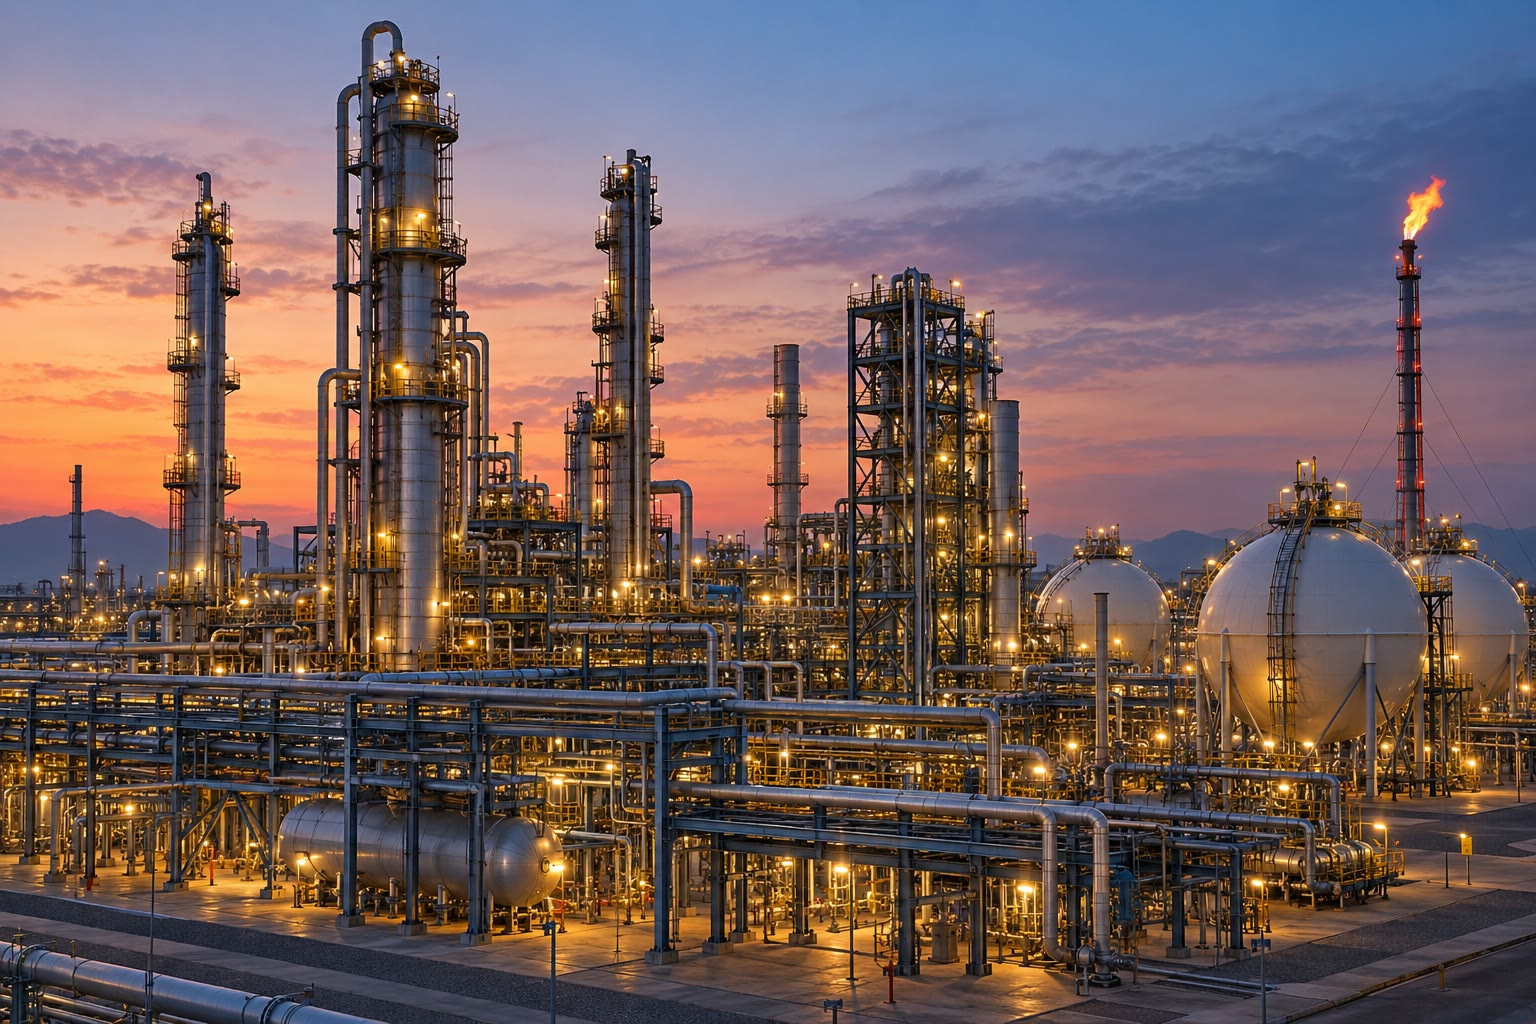
\includegraphics[width=0.6\linewidth]{images/book4/ai/b3-16-ammonia-plant.jpg}

{\small Sebuah pabrik sintesis amonia. Reaktor di jantungnya menampung
berton-ton katalis besi yang dipromosikan; sebagian besar pabrik itu
menyiapkan hidrogen dan mendaur ulang gas yang tidak terkonversi.}
\end{omfigure}

\section{Mengamati permukaan}

\begin{definition}[Spektroskopi desorpsi termal]\label{def:b3:surfaces-catalysis:tpd}
Pada \emph{spektroskopi desorpsi termal}\index{spektroskopi desorpsi termal},
permukaan yang membawa \omterm{def:b3:surfaces-catalysis:adsorption}{adsorbat} dipanaskan dengan laju tetap dan gas yang
terdesorpsi direkam dengan spektrometer massa; setiap keadaan ikatan
memberikan sebuah puncak, yang suhunya naik bersama energi aktivasi
\omterm{def:b3:surfaces-catalysis:adsorption}{desorpsinya}.
\end{definition}

Posisi sebuah puncak \omterm{def:b3:surfaces-catalysis:adsorption}{desorpsi} memberikan energi \omterm{def:b3:surfaces-catalysis:adsorption}{desorpsi} (untuk \omterm{def:b3:surfaces-catalysis:adsorption}{desorpsi} orde
satu, $E_d \approx RT_{\mathrm p}[\ln(\nu T_{\mathrm p}/\beta) - 3.64]$ dengan $\beta$ laju pemanasan dan $\nu \approx \qty{e13}{s^{-1}}$,
diterima tanpa bukti), dan luasnya memberikan jumlah yang teradsorpsi.
Spektroskopi fotoelektron sinar-X (XPS) mengukur energi ikat elektron-elektron
inti atom-atom permukaan, yang mengidentifikasi unsur-unsur dan bilangan
oksidasinya dalam beberapa nanometer pertama. Mikroskop \omterm{def:b3:quantum-model-systems:tunnelling}{penerowongan} pemindai
menggerakkan sebuah ujung yang runcing beberapa persepuluh nanometer di atas
permukaan penghantar; arus \omterm{def:b3:quantum-model-systems:tunnelling}{penerowongannya}
(\cref{ch:b3:quantum-model-systems}) turun sekitar satu orde besaran untuk
setiap \qty{0.1}{nm} jarak tambahan, sehingga dengan menjaga arus itu tetap
selama pemindaian, permukaan dapat dipetakan atom demi atom.

\begin{inthelab}[Sebuah pengukuran BET]
Sekitar \qty{0.2}{g} sampel ditimbang ke dalam tabung kaca berbola, dihilangkan
gasnya selama berjam-jam dalam vakum pada 150 sampai \qty{300}{\celsius}, ditimbang lagi, dan dipasang
pada instrumen, dengan bolanya terbenam dalam dewar berisi nitrogen cair.
Instrumen itu memasukkan nitrogen dalam takaran kecil dan mengukur tekanan
kesetimbangan sesudah setiap takaran, lalu menyimpulkan jumlah yang
teradsorpsi dari neraca gasnya; volume mati tabung diukur dengan helium, yang
tidak teradsorpsi.
\end{inthelab}

\begin{safety}{\ghs[0.7cm]{GHS06}\ghs[0.7cm]{GHS07}\ghs[0.7cm]{GHS08}\ghs[0.7cm]{GHS09}}
% ledger: ghs4:V2O5, ghs4:Ni
Katalis logam tereduksi (nikel, paladium, atau platina yang terbagi halus pada
penyangga, yang baru direduksi dalam hidrogen) dapat menyala bila bersentuhan
dengan udara: katalis itu ditangani di bawah gas inert dan dipasivasi sebelum
disimpan. Nikel adalah pemeka kulit dan diduga karsinogen; vanadium(V) oksida
beracun bila terhirup dan tertelan dan dapat menyebabkan kanker. Serbuk
katalis ditimbang di dalam ruang tertutup yang berventilasi.
\end{safety}

\begin{history}[Langmuir dan katalis amonia]
Irving Langmuir, yang bekerja pada bola lampu di sebuah laboratorium industri,
menurunkan isotermnya pada 1916--1918 dari gagasan bahwa gas yang teradsorpsi
membentuk lapisan setebal satu molekul, dan menerima Hadiah Nobel Kimia 1932
untuk kimia permukaannya. Beberapa tahun sebelumnya, Alwin Mittasch telah
mengorganisasi pencarian katalis amonia yang praktis: ribuan komposisi diuji
dalam reaktor-reaktor kecil bertekanan tinggi sebelum katalis besi yang
dipromosikan, yang masih dipakai sampai sekarang, dipilih. Itulah salah satu
penapisan katalis sistematis yang pertama.
\end{history}

\section{Latihan}

\begin{exercise}[$\star$]\label{exo:b3:surfaces-catalysis:1}
Sebuah gas menutupi 40\,\% sebuah permukaan Langmuir pada \qty{2.0}{kPa}. Hitunglah $K$ dan tutupannya pada
\qty{10}{kPa}.
\end{exercise}

\begin{exercise}[$\star$]\label{exo:b3:surfaces-catalysis:2}
Dua entalpi \omterm{def:b3:surfaces-catalysis:adsorption}{adsorpsi} diukur pada sebuah logam: $-20$ dan \qty{-150}{kJ/mol}. Manakah
yang \omterm{def:b3:surfaces-catalysis:physi-chemi}{fisisorpsi}, manakah yang \omterm{def:b3:surfaces-catalysis:physi-chemi}{kemisorpsi}? Manakah yang dapat bersifat disosiatif?
\end{exercise}

\begin{exercise}[$\star$]\label{exo:b3:surfaces-catalysis:3}
Hitunglah, per atom permukaan, situs puncak, jembatan, dan rongga pada muka (100) dan pada
muka (111) sebuah logam fcc.
\end{exercise}

\begin{exercise}[$\star$]\label{exo:b3:surfaces-catalysis:4}
Sebuah katalis mengonversi \qty{3.0e-6}{mol} pereaksi per gram per detik dan membawa
\qty{1.5e-5}{mol} situs permukaan per gram. Hitunglah frekuensi perputarannya.
\end{exercise}

\begin{exercise}[$\star\star$]\label{exo:b3:surfaces-catalysis:5}
Hidrogen teradsorpsi secara disosiatif dengan $\theta = 0.10$ pada \qty{1.0}{kPa}. Hitunglah $\theta$ pada \qty{4.0}{kPa}.
\end{exercise}

\begin{exercise}[$\star\star$]\label{exo:b3:surfaces-catalysis:6}
CO ($K = \qty{10}{kPa^{-1}}$) dan \ce{O2} ($K = \qty{0.5}{kPa^{-1}}$, tidak disosiatif dalam model sederhana ini)
bersaing memperebutkan situs permukaan platina pada 1.0 dan \qty{5.0}{kPa}. Hitunglah kedua
tutupannya dan berilah komentar tentang laju oksidasi CO.
\end{exercise}

\begin{exercise}[$\star\star$]\label{exo:b3:surfaces-catalysis:7}
Tutupan yang tercapai pada \qty{1.0}{kPa} pada \qty{300}{K} memerlukan \qty{8.0}{kPa} pada \qty{350}{K}. Hitunglah \omterm{def:b3:surfaces-catalysis:isosteric}{entalpi
adsorpsi isosteriknya}.
\end{exercise}

\begin{exercise}[$\star\star$]\label{exo:b3:surfaces-catalysis:8}
% ledger: sa:N2.am, const:Vm1, const:NA
Sebuah karbon aktif memiliki $v_{\mathrm m} = \qty{120}{cm^3.g^{-1}}$ (kondisi standar, 273.15 K dan
\qty{101.325}{kPa}). Hitunglah luas BET-nya.
\end{exercise}

\begin{exercise}[$\star\star$]\label{exo:b3:surfaces-catalysis:9}
Laju $\ce{2 CO + O2 -> 2 CO2}$ pada platina naik, melewati maksimum, lalu turun ketika $p(\ce{CO})$
bertambah pada $p(\ce{O2})$ tetap. Mekanisme manakah yang ditunjukkan oleh hal ini, dan mengapa CO
menginhibisi reaksinya?
\end{exercise}

\begin{exercise}[$\star\star\star$]\label{exo:b3:surfaces-catalysis:10}
Sebuah reaksi permukaan memiliki energi aktivasi sebenarnya \qty{100}{kJ/mol}; pereaksinya memiliki
$\Delta_{\mathrm{ads}}H = \qty{-60}{kJ/mol}$. Berapakah energi aktivasi yang terukur pada tutupan rendah dan pada tutupan
tinggi? Sketsalah $\ln r$ terhadap $1/T$ dalam rentang yang lebar.
\end{exercise}

\begin{exercise}[$\star\star\star$]\label{exo:b3:surfaces-catalysis:11}
Belerang teradsorpsi pada katalis nikel dengan tutupan 0.10 (atom belerang per
atom Ni permukaan), dan setiap atom belerang menyumbat empat situs. Berapakah
fraksi aktivitas yang tersisa untuk reaksi yang memerlukan satu situs bebas? Dan
untuk dua situs bebas yang bertetangga (anggaplah situs-situs yang tersumbat
tersebar secara acak)?
\end{exercise}

\begin{exercise}[$\star\star\star$]\label{exo:b3:surfaces-catalysis:12}
Untuk sintesis amonia, tiga logam mengikat atom nitrogen dengan entalpi
$-150$, $-250$, dan \qty{-400}{kJ/mol} (data latihan). Dengan \omterm{def:b3:surfaces-catalysis:sabatier}{asas Sabatier},
logam manakah yang mungkin merupakan katalis terbaik, dan apakah yang membatasi dua logam lainnya?
\end{exercise}

\section{Soal: Mengukur Sebuah Katalis}

\begin{problem}[{Soal akhir pekan --- mengukur sebuah katalis: luas BET katalis
platina berpenyangga, dispersi logam dan ukuran partikelnya dari kemisorpsi
hidrogen, dan frekuensi perputaran sebuah hidrogenasi}]
\label{pb:b3:surfaces-catalysis:1}
% ledger: sa:N2.am, lat:Pt, aw:Pt, const:Vm1, const:NA
Sebuah katalis mengandung 1.00\,\% massa platina pada alumina. Data soal:
isoterm nitrogen pada \qty{77}{K} (volume pada kondisi standar, 273.15 K dan
\qty{101.325}{kPa}, per gram):
\begin{center}\small
\begin{tabular}{lcccccc}
\hline
$x = p/p^*$ & 0.05 & 0.10 & 0.15 & 0.20 & 0.25 & 0.30 \\
$v$ / \unit{cm^3.g^{-1}} & 41.2 & 46.1 & 51.1 & 54.1 & 58.9 & 62.9 \\ \hline
\end{tabular}
\end{center}
\ce{H2} yang terkemisorpsi pada platina: \qty{0.205}{cm^3} per gram katalis. Sebuah hidrogenasi
berlangsung dengan laju \qty{2.0e-5}{mol} per gram katalis per detik. Platina: $M = \qty{195.08}{g/mol}$, fcc,
$a = \qty{392.3}{pm}$; volume molar gas pada kondisi standar \qty{22414}{cm^3/mol};
$a_{\mathrm m}(\ce{N2}) = \qty{0.162}{nm^2}$.

\medskip\noindent\textbf{Bagian I --- Plot BET.}
\begin{enumerate}[beginpenalty=10000]
  \item Mengapa isoterm itu diukur pada \qty{77}{K}?
  \item Mengapa hanya tekanan relatif antara 0.05 dan 0.30 yang dipakai?
  \item Hitunglah $x/(v(1 - x))$ untuk setiap titik.
  \item Garis kuadrat terkecilnya memiliki kemiringan \num{0.02205} dan perpotongan \num{0.000180} (dalam
        \unit{g.cm^{-3}}). Simpulkan $v_{\mathrm m}$.
  \item Simpulkan $c$. Apakah arti $c$ yang besar?
  \item Mengapa perpotongannya ditentukan dengan sangat buruk, dan apakah hal itu penting bagi $v_{\mathrm m}$?
\end{enumerate}

\medskip\noindent\textbf{Bagian II --- Luas.}
\begin{enumerate}[resume, beginpenalty=10000]
  \item Hitunglah jumlah nitrogen dalam \omterm{def:b3:surfaces-catalysis:coverage}{lapisan tunggal} per gram.
  \item Hitunglah \omterm{def:b3:surfaces-catalysis:surface-area}{luas permukaan spesifiknya}.
  \item Bagian padatan manakah yang menyediakan hampir seluruh luas ini?
  \item Mengapa metode BET gagal untuk padatan mikropori seperti zeolit?
\end{enumerate}

\medskip\noindent\textbf{Bagian III --- Dispersi dan ukuran partikel.}
\begin{enumerate}[resume, beginpenalty=10000]
  \item Hitunglah jumlah atom H yang terkemisorpsi per gram.
  \item Hitunglah jumlah platina per gram.
  \item Simpulkan dispersinya.
  \item Hitunglah volume per atom Pt di bagian dalam padatan.
  \item Luas per atom permukaan, yang dirata-ratakan atas muka (111), (100), dan (110),
        adalah \qty{0.0807}{nm^2}. Periksalah nilai untuk (111), $\frac{\sqrt3}{4}a^2$.
  \item Tunjukkan bahwa untuk bola $d = 6v_{\mathrm{at}}/(a_{\mathrm{at}}D)$.
  \item Hitunglah diameter partikel rata-rata.
  \item Asumsi-asumsi manakah yang membatasi hasil ini?
\end{enumerate}

\medskip\noindent\textbf{Bagian IV --- Aktivitas.}
\begin{enumerate}[resume, beginpenalty=10000]
  \item Hitunglah frekuensi perputaran per atom Pt permukaan.
  \item Hitunglah laju per gram platina.
  \item Jika partikel-partikelnya mengalami \omterm{def:b3:surfaces-catalysis:catalyst-design}{sintering} sampai \qty{10}{nm} pada frekuensi perputaran
        yang tetap, dengan faktor berapakah laju per gram akan turun?
  \item Apakah yang diungkapkan oleh frekuensi perputaran yang berubah bersama ukuran partikel?
  \item Mengapa katalis dibandingkan berdasarkan frekuensi perputaran dan bukan
        berdasarkan laju per gram?
  \item Nyatakan hasilnya: diameter rata-rata partikel platina.
\end{enumerate}
\end{problem}
